\documentclass[11pt]{article}

\usepackage[margin=1in]{geometry}
\usepackage{amsmath}
\usepackage{amssymb}
\usepackage{graphicx}
\usepackage{xcolor}
\usepackage[hidelinks]{hyperref}

\newcommand{\code}[1]{\texttt{#1}}

\title{Risk-Governed On-Chain DeFi Agents:\\
Deterministic, Regime-Aware Position Sizing Under Real Execution Frictions}
\author{Utku Egemen Umut}
\date{August 2026}

\begin{document}
\maketitle

\begin{abstract}
Most crypto trading agents built on large language models (LLMs) focus on two questions: what to
trade and how to execute it. The question of \emph{how much} to risk, given the current market
regime, is usually left to the model or to a fixed rule. This whitepaper describes a small Ethereum
DeFi agent, built on the ElizaOS ``Spartan'' framework, that adds a deterministic risk-governance
layer between the language model and execution. The layer sizes positions with volatility targeting,
fractional-Kelly shrinkage, and a hard wallet cap, and it refuses Aave borrows that would push the
projected health factor below a floor. The sizing arithmetic never runs through the LLM. We verify
the execution engine (Uniswap~V2 swaps, ERC-20/ETH transfers, Aave~V3 supply/borrow) on a mainnet
fork with real transaction hashes, and we run a small, no-lookahead sizing backtest on one year of
ETH prices to illustrate the layer's behavior. Our contribution is a proposal and a first
implementation, not a result proven at scale; we picked up most of these ideas recently and treat
the evaluation accordingly. On a two-month stretch of high volatility, volatility targeting cut
realized volatility from about 88\% to 60\% per year and reduced maximum drawdown from 43\% to 35\%
relative to holding ETH, without claiming any excess return.
\end{abstract}

\section{Introduction and the gap}\label{sec:intro}
Two recent lines of work frame the problem we care about. \textbf{CryptoBench}~\cite{cryptobench}
evaluates LLM agents on expert-curated cryptocurrency analysis and finds a sharp split: agents
retrieve facts well but are weak at prediction, with the best complex-prediction score around
$18.6\%$. \textbf{LLM multi-agent portfolio management}~\cite{mas} backtests a team of
modality-specialized agents and reports strong returns for the best configuration (about $+133.5\%$
at a Sharpe of $1.50$ over its test period), but it abstracts away slippage and price impact and does
not solve regime switching: its best full-period, best-bull, and best-bear configurations are three
different setups, chosen after the fact.

Newer trading-focused benchmarks reinforce the same lesson. \textbf{AI-Trader}~\cite{aitrader}, a
live, contamination-controlled benchmark across stocks, A-shares, and crypto, reports that general
intelligence does not translate into trading skill and that \emph{risk-control capability} is what
determines robustness across markets. \textbf{When Agents Trade}~\cite{ama} and
\textbf{InvestorBench}~\cite{investorbench} draw similar distinctions between agent frameworks, with
behavior ranging from aggressive to conservative largely driven by the surrounding framework rather
than the model backbone.

The pattern we build on is well known. Direction is close to unforecastable, but volatility is more
forecastable: it clusters and is autocorrelated. An agent that is right on direction but three times
oversized into a volatility spike still loses. So the useful lever is not better prediction; it is
disciplined sizing that leans on the forecastable quantity and respects real execution costs. That
sizing-relative-to-regime layer is the part most projects skip, and it is where we try to
contribute.

\paragraph{Scope and honesty.} This is a whitepaper, not a rigorous study. We are recent learners of
these methods, not experts. Every claim below is meant to be proportional to its evidence: the
execution engine is verified on a fork with real transaction hashes, and the sizing layer is
demonstrated with unit tests and one illustrative backtest. We do not claim profitability, statistical
significance, or that the design generalizes.

\section{System}\label{sec:system}
The agent is the ElizaOS ``Spartan'' project adapted to Ethereum. The Ethereum logic lives in a
custodial wallet plugin (\code{src/plugins/multiwallet}). A single file, \code{utils/ethereum.ts},
holds the viem-based execution engine: address and key handling, Uniswap~V2 swaps with automatic
allowance and slippage handling, native and ERC-20 transfers, and Aave~V3 supply and borrow.

A user imports a wallet in chat, and the agent detects the key, derives the address, and stores it.
Chat commands (``swap 0.05 ETH to USDC'', ``supply 100 USDC to Aave'') are parsed by the LLM into a
structured intent, which is then executed by the deterministic engine. We test against a local
mainnet fork (Foundry Anvil), which keeps the hardcoded mainnet contract addresses and real liquidity
working while risking no real funds.

On top of this sits the risk-governance layer (\code{src/plugins/multiwallet/risk}), added as three
ElizaOS surfaces backed by one service:
\begin{itemize}
  \item a \textbf{service} that computes the current regime (realized volatility), the
        volatility-targeted maximum position, and the Aave borrow headroom;
  \item a \textbf{context provider} that injects that budget into the agent on every turn, so the
        model is aware of its limits and does not propose oversized trades; and
  \item pre-execution \textbf{guards} on the swap and borrow paths that clamp or refuse a request
        that violates the budget, plus a read-only advisory action that answers ``how much can I
        safely swap or borrow?''.
\end{itemize}
The important design choice is that the model proposes intent and reads the regime qualitatively, but
the multiply-by-size step is deterministic code.

\section{Method}\label{sec:method}
The math here is deliberately modest. We reuse standard results and keep the derivations short.

\subsection{Uniswap V2 execution and price impact}
Uniswap~V2 holds reserves $(x, y)$ of two tokens on a constant-product curve $x \cdot y = k$. With the
$0.30\%$ fee, swapping an input $\Delta x$ returns
\begin{equation}
\Delta y \;=\; \frac{997\,\Delta x\, y}{1000\,x + 997\,\Delta x}.
\end{equation}
The realized (execution) price $p_{\text{exec}} = \Delta y / \Delta x$ is worse than the spot price
$p_{\text{spot}} = y/x$, and the gap grows with trade size. We define price impact as
\begin{equation}
\text{impact}(\Delta x) \;=\; 1 - \frac{p_{\text{exec}}}{p_{\text{spot}}},
\end{equation}
and the engine protects the trade with a slippage tolerance $s$, submitting a minimum-output bound
$y_{\min} = \hat{y}\,(1-s)$ where $\hat{y}$ is the quoted output.

\subsection{Aave health factor and a borrow floor}
For a borrower with collateral values $C_i$, per-asset liquidation thresholds $\lambda_i \in [0,1]$,
and total debt $D$, the Aave health factor is
\begin{equation}
\mathrm{HF} \;=\; \frac{\sum_i C_i\,\lambda_i}{D}.
\end{equation}
A position is liquidatable once $\mathrm{HF} < 1$. We enforce a floor $H_{\text{floor}}$ (default
$1.5$): a prospective borrow of base value $b$ is refused unless the projected health factor
$\big(\sum_i C_i \lambda_i\big)/(D + b) \ge H_{\text{floor}}$. Inverting this gives the largest safe
additional borrow,
\begin{equation}
b^{*} \;=\; \max\!\left(0,\ \frac{\sum_i C_i\,\lambda_i}{H_{\text{floor}}} - D\right),
\label{eq:maxborrow}
\end{equation}
which the advisory action reports directly.

\subsection{Volatility targeting and fractional Kelly}
Let $r_t = \ln(p_t / p_{t-1})$ be log returns over a trailing window. The annualized realized
volatility is
\begin{equation}
\hat{\sigma} \;=\; \sqrt{P}\;\cdot\;\mathrm{std}(r_t),
\end{equation}
with $P$ the number of periods per year ($P=365$ for daily data). Volatility targeting sets the
position as a fraction of the wallet so that its risk matches a target $\sigma_{\text{target}}$:
\begin{equation}
f_{\text{vol}} \;=\; \frac{\sigma_{\text{target}}}{\hat{\sigma}}.
\end{equation}
As realized volatility rises, the fraction shrinks. Independently, the fractional-Kelly fraction for
an edge $\mu$ and variance $\sigma^2$, shrunk by $\lambda \in (0,1]$, is
\begin{equation}
f_{\text{Kelly}} \;=\; \lambda\,\frac{\mu}{\sigma^2}.
\end{equation}
The engine takes the most conservative of the three constraints, including a hard wallet cap $c$:
\begin{equation}
f \;=\; \min\big(f_{\text{vol}},\ f_{\text{Kelly}},\ c\big).
\label{eq:min}
\end{equation}
When no edge estimate is available, the Kelly term is set aside and sizing rests on volatility and the
cap alone.

\subsection{Sizing under slippage}
Combining sizing with price impact gives a small optimization. If a trade of size $q$ has expected
per-unit edge $\mu$ and the constant-product curve produces impact that is approximately linear in $q$
near the current reserves (so total impact cost is roughly $\kappa q^2$), the expected net value is
\begin{equation}
V(q) \;=\; \mu\,q - \kappa\,q^{2},
\end{equation}
which is concave and maximized at $q^{*} = \mu/(2\kappa)$. The point is qualitative: the larger the
trade relative to pool depth, the more impact erodes the edge, so the size that is optimal net of
frictions is smaller than the size a frictionless model would choose. Our implementation does not
solve this in closed form; it clamps to the volatility- and cap-based budget, which is the binding
constraint in the regimes we tested.

\section{Contribution}\label{sec:contribution}
The contribution is a deterministic, regime-aware risk-governance layer for an on-chain LLM agent,
evaluated under real execution frictions rather than in an idealized simulator. Three points
distinguish it from the prior work in Section~\ref{sec:intro}:
\begin{enumerate}
  \item \textbf{The LLM is kept out of the sizing arithmetic.} It proposes intent and reads the
        regime; rules compute the number. This removes a class of errors where a model over- or
        under-sizes a trade.
  \item \textbf{Sizing leans on the forecastable quantity.} Following the retrieval-versus-prediction
        gap in CryptoBench~\cite{cryptobench} and the risk-control finding in AI-Trader~\cite{aitrader},
        we size on volatility rather than on a predicted direction.
  \item \textbf{Execution frictions are real, not assumed away.} The multi-agent portfolio
        work~\cite{mas} abstracts slippage; here swaps, transfers, and Aave interactions run against
        real mainnet contracts on a fork, and the borrow guard reads live Aave account state.
\end{enumerate}
We frame this as a proposal plus a first implementation. It is not a proof that the design improves
live trading outcomes.

\section{Results}\label{sec:results}
All numbers below come from artifacts in the repository; none are invented.

\subsection{Execution engine, verified on a mainnet fork}
Running the full pipeline against an Anvil mainnet fork produced real transactions. Table~\ref{tab:tx}
lists the confirmed hashes; every receipt has status success. Two batches are shown: a scripted
end-to-end smoke test on a fresh fork, and the chat-driven flow where the agent fired the actions
itself. A live, read-only call against Ethereum mainnet through the same code returned a Uniswap~V2
quote of $1\,\text{WETH} \rightarrow 1876.30\ \text{USDC}$, confirming the read path against real
liquidity.

\begin{table}[h]
\centering
\small
\begin{tabular}{l l l}
\hline
Source & Flow & Transaction hash (truncated) \\
\hline
Smoke test & Transfer (native ETH)        & \code{0xc523e4f5\ldots46883} \\
Smoke test & Swap ETH $\rightarrow$ USDC  & \code{0x04bbdc3d\ldots77c61} \\
Smoke test & Aave supply USDC             & \code{0x277510c2\ldots42b6c} \\
Smoke test & Aave borrow DAI              & \code{0x5774d1bd\ldots9a882} \\
Chat-driven & Swap ETH $\rightarrow$ USDC & \code{0x99b65f21\ldots57d04} \\
Chat-driven & Swap ETH $\rightarrow$ USDC & \code{0xee1a4695\ldots90ec9} \\
Chat-driven & Aave supply USDC            & \code{0x765bce00\ldots7cc2c} \\
\hline
\end{tabular}
\caption{On-chain transactions produced on the Anvil mainnet fork (all status success).}
\label{tab:tx}
\end{table}

\subsection{Deterministic sizing and the health-factor floor}
The risk layer answers sizing queries directly. For a wallet holding roughly $9999.9$~ETH with ETH
realized volatility around $39\%$ per year (live), the volatility-targeted budget is capped by the
$25\%$ wallet limit at about $2499.97$~ETH. For a wallet with $\$187.63$ of Aave collateral and no
debt, Equation~\eqref{eq:maxborrow} gives a safe additional borrow of $\$97.57$ at the $1.5$ floor; a
request to borrow $\$300$ is refused because the projected health factor falls to $0.49$. These values
are reproduced by unit tests over the pure sizing functions.

\subsection{Illustrative sizing backtest}
To show how the layer behaves over time we ran a deterministic, no-lookahead backtest on one year of
daily ETH prices (13 August 2025 to 12 August 2026), a period in which ETH fell about $58\%$. The
structure borrows from live-agent benchmarks such as AMA~\cite{ama} and AI-Trader~\cite{aitrader}: at
each day the policy sees prices only up to that day, chooses an exposure, and that exposure is applied
to the next day's return, with a simple turnover cost. The decision-maker is our deterministic sizing
layer, not the LLM. We compare four policies: buy-and-hold, a fixed half-exposure, volatility
targeting, and volatility targeting with a full-exposure cap.

Figure~\ref{fig:ablation} and Table~\ref{tab:backtest} report the most volatile 60-day window, where
the effect is clearest. Volatility targeting cut annualized realized volatility from $87.6\%$
(buy-and-hold) to about $60\%$, and reduced maximum drawdown from $42.8\%$ to $35.5\%$. In the calmest
60-day window (not shown) the volatility-targeted policies stayed near full exposure and tracked
buy-and-hold closely, which is the intended behavior: pull risk in when volatility is high, leave it
on when volatility is low. Fixed half-exposure achieves low volatility trivially by always investing
half; unlike volatility targeting, it does not adapt to the regime.

\begin{figure}[h]
\centering
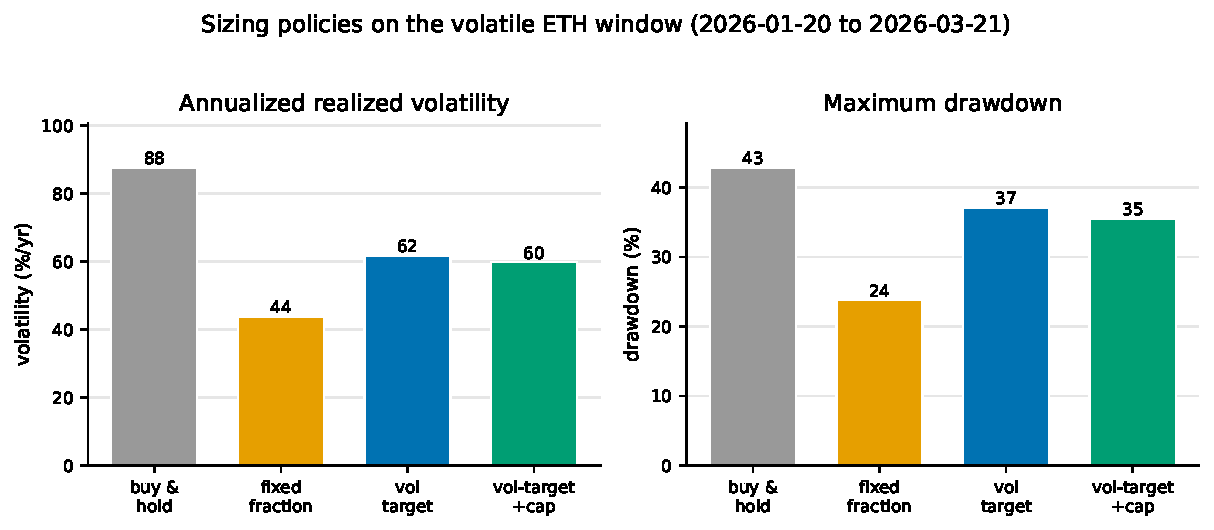
\includegraphics[width=\textwidth]{figures/sizing_ablation.pdf}
\caption{Sizing policies on the most volatile 60-day ETH window. Volatility targeting (with and
without a full-exposure cap) lowers realized volatility and drawdown relative to buy-and-hold, while
fixed half-exposure does so only by holding a constant half position.}
\label{fig:ablation}
\end{figure}

\begin{table}[h]
\centering
\small
\begin{tabular}{l r r r r}
\hline
Policy & Ann.\ vol & Max drawdown & Sharpe & Excess vs.\ hold \\
\hline
Buy-and-hold      & $87.6\%$ & $-42.8\%$ & $-2.31$ & $\phantom{+}0.0\%$ \\
Fixed fraction    & $43.8\%$ & $-23.8\%$ & $-2.31$ & $+16.1\%$ \\
Volatility target & $61.7\%$ & $-37.1\%$ & $-3.05$ & $+3.8\%$ \\
Vol.\ target + cap& $59.9\%$ & $-35.5\%$ & $-2.92$ & $+5.5\%$ \\
\hline
\end{tabular}
\caption{Backtest metrics on the volatile window. Sharpe is negative for all policies because ETH
fell over the period; the point is volatility and drawdown control, not return.}
\label{tab:backtest}
\end{table}

We read these results narrowly. Volatility targeting does what it is designed to do, which is control
realized volatility and drawdown, not generate return. Over the full bear year, plain fixed-fraction
sizing had the best return simply because it stayed less exposed; that is not evidence for any policy's
skill, only for lower exposure in a falling market.

\subsection{Related work and where our evaluation falls short}
Recent surveys of LLM trading agents are blunt about evaluation quality. A review of 77
studies~\cite{survey} finds that within the subset that even runs a closed-loop evaluation, only about
$10.5\%$ report time-consistent train/test splits and only about $5.3\%$ report an explicit cost
model; a companion audit~\cite{execreview} reaches the same conclusion about execution realism. Read
against that checklist, our backtest satisfies some items (no lookahead, a turnover cost, a bundled
price series for exact reproducibility) and clearly fails others (a single asset, single windows, no
multi-seed robustness, and no out-of-sample testing). We report it as an illustration, in the spirit
those surveys recommend: preliminary unless supported by stronger evidence. Standardized benchmarks
such as InvestorBench~\cite{investorbench}, STOCKBENCH~\cite{stockbench}, and
CryptoTrade~\cite{cryptotrade} are the natural next targets for a fuller evaluation.

\section{Limitations and reproducibility}\label{sec:limits}
The honest caveats are as follows. A fork is not live trading: state is pinned, there are no
adversarial counterparties, and MEV is absent. The backtest is one asset over one year with single
windows and a single seed. The agent's action selection is non-deterministic: even when a wallet
action is valid, the model sometimes replies conversationally instead of firing it, so a command may
need to be repeated. The borrow guard values new debt at roughly one dollar per token, which is
accurate for the stablecoin borrows we tested but not in general. And, as stated up front, we are
new to this material.

Everything is reproducible. The setup runbook is in \code{docs/SETUP\_FROM\_SCRATCH.md}; the pure
sizing functions have unit tests (\code{bun test src/plugins/multiwallet/risk}); the read-only demo,
the fork smoke test, the risk demo, and the backtest are scripts in \code{scripts/}; and the backtest
ships with the exact ETH price series it used so its numbers can be regenerated offline.

Future work is the part we have not earned yet: a multi-seed, multi-asset, out-of-sample evaluation
against a standardized benchmark; a live-agent variant where the model is in the decision loop; richer
regime inputs (funding, open interest, on-chain flows, macro); and MEV-protected execution for larger
orders.

\begin{thebibliography}{99}
\bibitem{cryptobench} J.\ Guo et al. \emph{CryptoBench: A Dynamic Benchmark for Expert-Level
Evaluation of LLM Agents in Cryptocurrency.} arXiv:2512.00417, 2025.
\bibitem{mas} Y.\ Luo et al. \emph{LLM-Powered Multi-Agent System for Automated Crypto Portfolio
Management.} arXiv:2501.00826, 2025.
\bibitem{ama} \emph{When Agents Trade: Live Multi-Market Trading Benchmark for LLM Agents (Agent
Market Arena).} arXiv:2510.11695, 2025.
\bibitem{aitrader} T.\ Fan, Y.\ Yang, Y.\ Jiang, et al. \emph{AI-Trader: Benchmarking Autonomous
Agents in Real-Time Financial Markets.} arXiv:2512.10971, 2025.
\bibitem{investorbench} H.\ Li, Y.\ Cao, Y.\ Yu, et al. \emph{InvestorBench: A Benchmark for
Financial Decision-Making Tasks with LLM-based Agent.} ACL 2025; arXiv:2412.18174, 2024.
\bibitem{stockbench} \emph{STOCKBENCH: Can LLM Agents Trade Stocks Profitably in Real-World Markets?}
arXiv:2510.02209, 2025.
\bibitem{survey} Y.\ Xia, P.\ You, T.\ Wang, et al. \emph{Agentic Trading: When LLM Agents Meet
Financial Markets.} arXiv:2605.19337, 2026.
\bibitem{execreview} J.\ Yao and Z.\ Zheng. \emph{Beyond Agent Architecture: Execution Assumptions and
Reproducibility in LLM-Based Trading Systems.} arXiv:2606.08285, 2026.
\bibitem{cryptotrade} \emph{CryptoTrade: A Reflective LLM-based Agent to Guide Zero-shot
Cryptocurrency Trading.} Findings of EMNLP, 2024.
\bibitem{uniswapv2} H.\ Adams, N.\ Zinsmeister, D.\ Robinson. \emph{Uniswap v2 Core.} Technical
whitepaper, 2020.
\bibitem{aavev3} Aave. \emph{Aave V3 Technical Paper.} 2022.
\bibitem{kelly} J.\ L.\ Kelly Jr. \emph{A New Interpretation of Information Rate.} Bell System
Technical Journal, 35(4):917--926, 1956.
\bibitem{moreira} A.\ Moreira and T.\ Muir. \emph{Volatility-Managed Portfolios.} Journal of Finance,
72(4):1611--1644, 2017.
\end{thebibliography}

\end{document}
